\subsection{Worst-Case Approximation}
The results in the previous section concentrated on producing nearly
optimal solutions in expectation. In this section, we will show that
it is possible to obtain good solutions regardless of the model that
generated the recommendation subgraph. As usual we let $G=(L,R,E)$ be a
bipartite graph on which we would like to solve the $(c,a)$-graph
recommendation problem and consider the following greedy
algorithm. Consider each vertex in $R$ in some arbitrary order and if
there is some $v \in R$ that has $a$ neighbors in $L$ all of which
have degree $< c$, add the edges to these neighbors to $H$. If there
are any ties about the nodes to be picked either in the selection of
$v$ or its neighbors, we can break ties arbitrarily. This algorithm
has the following approximation guarantee

\begin{thm}
The greedy algorithm described above achieves a $1/(a+1)$-approximation ratio.
\end{thm}
\begin{proof}
Let $R_{GREEDY}, R_{OPT}\subseteq R$ be the set of vertices that have
degree $\geq a$ in the greedy and optimal solutions respectively. Note
that any $v \in R_{OPT}$ along with neighbors $\{u_1,\ldots u_a\}$
forms a set of candidate edges that can be taken by the greedy
algorithm. So we can consider $R_{OPT}$ as a candidate pool for
$R_{GREEDY}$. Each move that the greedy algorithm makes might make
some of the candidates infeasible, but as long as the candidate pool
is not depleted, the greedy algorithm can continue adding vertices to
its solution. Each time the greedy algorithm claims some vertex $v\in
R$ with edges to $\{u_1,\ldots, u_a\}$, we have obviously have to
remove $v$ from the candidate pool. If any $u_i$ was saturated
(i.e. had degree $c$) in the optimal solution, we would also need to
remove an arbitrary vertex $v_i\in R$ adjacent to $u_i$ in the optimal
solution. In other words, by using an edge of $u_i$, we force it to
not use an edge it used to some other $v_i$, which might cause the
degree of $v_i$ to go below $a$. (Note that the greedy algorithm does
not actually have to be aware of the structure of optimal solution for
this type of bookkeeping to go through.) Therefore, at each step of
the greedy algorithm, we have to remove at most $a+1$ vertices from
the candidate pool. Since our candidate pool has size $OPT$, the
greedy algorithm cannot stop before it has added $|OPT|/(a+1)$
vertices to the solution.
\end{proof}

\begin{figure}[h]
\centering
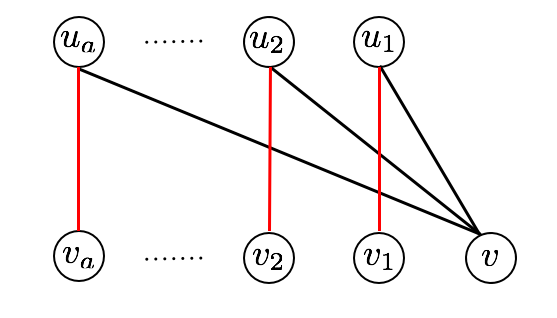
\includegraphics[width=.5\textwidth]{greedy.png}
\begin{minipage}[h]{.8\linewidth}
\caption{This diagram shows one step of the greedy algorithm. When $v$ claims edges to $u_1,\ldots, u_a$, it potentially removes $v_1,\ldots, v_a$ from the pool of candidates that are avaiable. The potentially invalidated edges are shown in red.}
\end{minipage}
\end{figure}

There are twp things to note about this algorithm. The first is
that the solution the greedy algorithm outputs is dependent on the
order the vertices in $R$ are processes. It may be possible to improve
the expected approximation ratio by permuting these vertices randomly
before the algorithm runs. The second is that this approximation
guarantee is as good as we can expect. In particular, if we set $a=1$
then we obtain the familiar $1/2$-approximation for matchings.

\label{worst-vs-avg}